\documentclass[10pt]{article}
\usepackage[margin=18mm]{geometry}
\usepackage{graphicx,booktabs,hyperref}
\usepackage[strings]{underscore}
\setlength{\parindent}{0pt}\setlength{\parskip}{5pt}
\begin{document}
\section*{Supported quartic continuation: interrupted runs and checked answers}

Original additional L0 runs began 2026-10-25 at 17:54:16 UTC (m14) and
22:49:42 UTC (m15). Same registered eight one-target workloads and three
arms, frozen ecbench source 0a5137c2, binary SHA prefix efa25f209e57.
Shared AMD EPYC 9V74 host, four Rayon threads, 12-GiB address space,
1,800 seconds per arm and 14,400 seconds outer cap per run/replay.
Wall/CPU time is diagnostic; these do not replace the original L2 ladder.

\begin{center}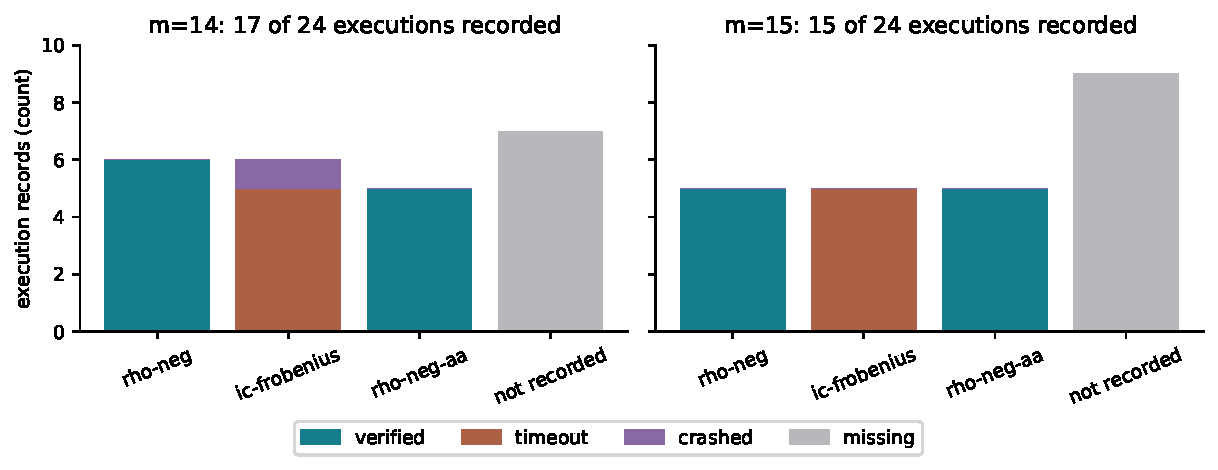
\includegraphics[width=\linewidth]{partial-quartic-outcomes.pdf}\end{center}
m14 retains 17/24 records: 11 successful rho answers, five IC timeouts and
one interrupted/crashed IC attempt, with seven registered executions missing.
Its original native audit binds all files and reproduces the 11 successful
records byte-identically, but returns failure because the session is
interrupted. m15 retains 15/24 records: ten successful rho answers and five
IC timeouts, with nine executions missing. It has no completed-session or
all-record replay certificate. The environment restart left no live runner.

The new native audit independently verifies every one of those 11 and ten
successful scalars with BinaryCurve arithmetic, using the exact recorded
generator and target. Curve identity, subgroup/order and generator checks
agree with the reconstructed model. Legacy point coordinates use the packed
tower basis; the adapter converts them to the canonical polynomial basis.
Two initial verifier failures from misreading that encoding are preserved;
the corrected audit repeats byte-identically. The factories' generators
agree after the coordinate conversion on both checked models.

\textbf{Limits.} No IC attempt in these retained records completed.
Missing/censored work has unknown cost; no successful-only cost mean or
IC/rho ratio is computed. Answer checks are not new rho walks, independent
counter recounts, or a completed session. Original L2 m14/15, full wide IC
adapters and the 124-branch independent HKY program remain unresolved.

\begin{flushleft}\footnotesize
Exact curve/subgroup models: \texttt{../../curve-identity-adapter.v2.json}.\par
Native receipt: \texttt{../../pipeline-receipts/publication-followup-audit-v3-20261026/output.json}.\par
Protocol: FOLLOWUP_PUBLICATION_AUDIT_PROTOCOL.md; preserved original SUPPORTED_LOCAL_QUARTIC_PROTOCOL.md.\par
Archive: evidence/runs-partial-quartics-complete-20261026.tar.xz.\par
No measured crossover, complete-price IC gain, or artifact-store upload is inferred.
\end{flushleft}

\end{document}
